\begin{appendix}

%-----------------------------------------------------------------------------
\chapter{Latex Examples}
%-----------------------------------------------------------------------------

%-----------------------------------------------------------------------------
\section{Text Typesettings}
%-----------------------------------------------------------------------------

Test {\it Test} {\bf Test} {\tt Test} {\sc Test}

\tiny{Test} \small{Test} \normalsize{Test} \large{Test} \Large{Test}
\LARGE{Test} \huge{Test} \Huge{Test}
\normalsize{Test}

\begin{center}
This is a text. 
\end{center}

\begin{flushleft}
This is a text.
\end{flushleft}

\begin{flushright}
This 
is 
a 
text.

\end{flushright}

\begin{verbatim}
    #ifndef _MYFILENAME_IDL_
    #define _MYFILENAME_IDL_
    
    // some IDL definitions

    #endif /* _MYFILENAME_IDL_ */
\end{verbatim}

\newpage

%-----------------------------------------------------------------------------
\section{Enumerations}
%-----------------------------------------------------------------------------

\begin{itemize}
  \item one
  \item two
  \item three
  \begin{itemize}
    \item a
    \item b
    \item c
  \end{itemize}
\end{itemize}

\begin{enumerate}
  \item one
  \item two
  \item three
\end{enumerate}


\begin{description}
\item[one] blah
\item[two] blah blah
\item[three] blah blah blah
\end{description}

\newpage


%-----------------------------------------------------------------------------
\section{Tables}
%-----------------------------------------------------------------------------

We can refer to existing tables like (see Tab.~\ref{UserTable}).

\begin{table}[htbp]
\begin{center}
\begin{tabular}{|r||l|c|} 
\hline 
ID 	& Username 	& Password 	\\ 
\hline 
\hline
3 	& Eva 		& xxx 		\\ 
\hline
5 	& Willi 	& xxx 		\\ 
\hline
\end{tabular}
\end{center}
\caption{An example table.}
\label{UserTable}
\end{table}

\newpage


%-----------------------------------------------------------------------------
\section{Footnotes}
%-----------------------------------------------------------------------------
We can add a footnote\footnote{Some footnotes.}  to a text.


\newpage


%-----------------------------------------------------------------------------
\section{Mathematical Expressions}
%-----------------------------------------------------------------------------

Simple mathematical expressions like $z=a+jb$ can be embedded directly into the
text.

\begin{displaymath}
y=\frac{1}{x+1}
\end{displaymath}


\begin{displaymath}
abs = \sqrt{re^2 + im^2}
\end{displaymath}

\begin{displaymath}
\int_{a}^{b} f(x)g(x)dx
\end{displaymath}

\newpage


%-----------------------------------------------------------------------------
\section{Pictures}
%-----------------------------------------------------------------------------

We can refer to a picture like (see Fig.~\ref{ComponentDef}) to
add a more detailed description in the text.

\begin{figure}[htbp]
    \centering
    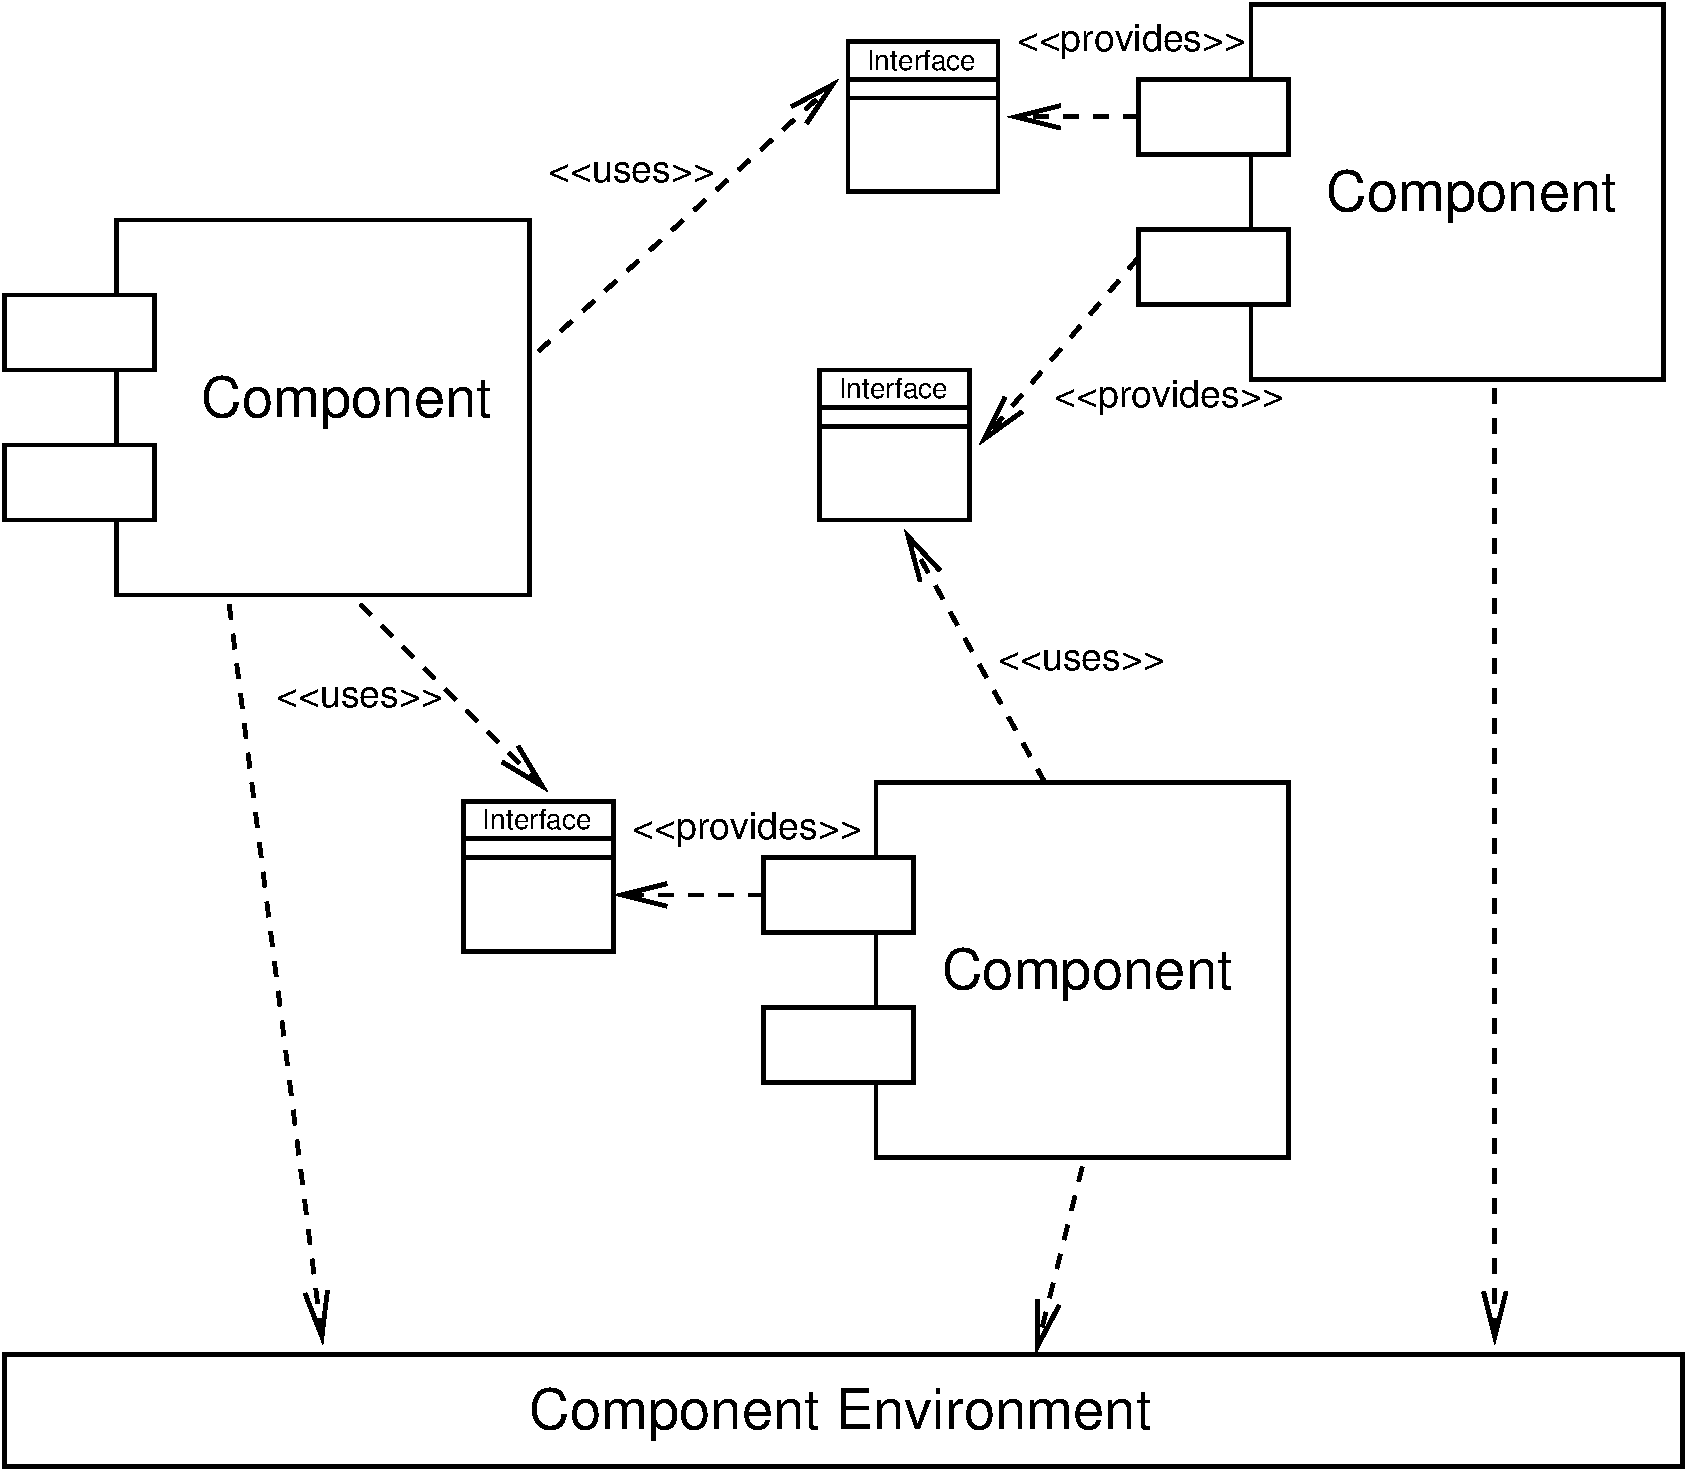
\includegraphics [width=8cm,angle=30] {figures/Environment}
    \caption{A software component is a unit of composition with 
        contractually specified interfaces and explicit context 
		dependencies only.}
    \label{ComponentDef}
\end{figure}



%-----------------------------------------------------------------------------
\section{Citations}
%-----------------------------------------------------------------------------

The foundation of a solid software design are design patterns.
Beside of the GoF book \cite[S. 190]{Gamma95} there are many other books to this
topic \cite[S. 999]{Marinescu02} \possessivecite{dpquiz}
\cite{Wick2005} \cite{Gamma95}.

\end{appendix}
